\def\firstname{firstname}
\def\lastname{lastname}
\def\aufgabenblatt{4}
\documentclass{article}

\usepackage[a4paper, margin=2.5cm]{geometry}
\usepackage{graphicx}
\usepackage[ngerman]{babel} % automatische Silbentrennung
\usepackage[table]{xcolor}
\usepackage{tabularx,array,booktabs,makecell}
\usepackage{titlesec}
\usepackage{amsmath}

\usepackage{fancyhdr}
\pagestyle{fancy} 
\fancyhead[L]{\firstname \: \lastname\\}  
\fancyhead[C]{Bildverarbeitung und Mustererkennung\\Aufgabenblatt \aufgabenblatt}
\fancyhead[R]{\\
\includegraphics[width=0.25\textwidth]{../common/hs_aalen_de.png}}

\fancypagestyle{page1}{
	\fancyhead[L]{\firstname \: \lastname\\}
	\fancyhead[C]{Bildverarbeitung und Mustererkennung\\Aufgabenblatt \aufgabenblatt}
	\fancyhead[R]{ \\
\includegraphics[width=0.25\textwidth]{../common/hs_aalen_de.png}}

}
\setlength{\parindent}{0mm}
\setlength{\parskip}{2.5mm}

\titlespacing*{\section}{0mm}{4pt}{0pt}
\setlength{\headsep}{14mm}

\begin{document}

\thispagestyle{page1} 

\section{Constructing Convolution Kernel}

In this exercise, we will use convolutions to distort images. Edit the file \texttt{convolution.ipynb}.

\subsection{Gaussian Filter}

\begin{enumerate}

\item[a)] Construct a gaussian filter with $\sigma=3.0$ and convolve the file \texttt{images/kodim15.png} using this kernel. 
\begin{center}
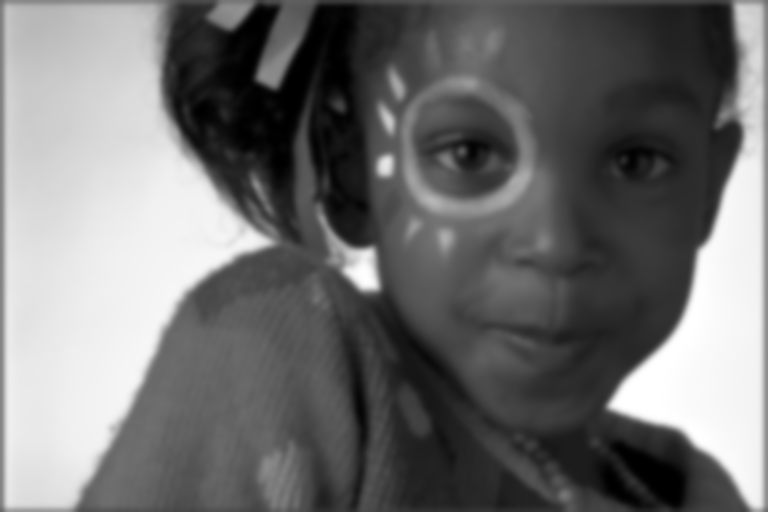
\includegraphics[width=0.45\textwidth]{source\_code/kodim15_a.png}
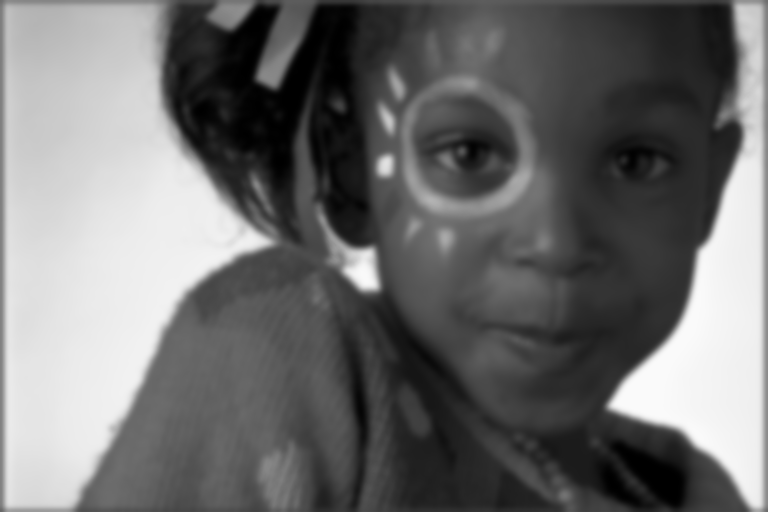
\includegraphics[width=0.45\textwidth]{source\_code/kodim15_a_result.png}
\end{center}

\item[b)] What kernel size did you choose and why?
\item[c)] Visualize the fourier spectrum (magnitude) of the original image, the kernel, and the convolution result.

\end{enumerate}

I needed the following time to complete the task:

\section{Estimating Convolution Kernel}

In this exercise, we will estimate kernels that were used to distort images. You may use various techniques to do so.

\begin{enumerate}

\item[a)] The file \texttt{images/kodim15b.png} was distorted with some sort of directional blurr filter. Estimate the parameters of the filter as precisely as possible.
\item[b)] Describe the procedure you used for estimating the distortion. \\
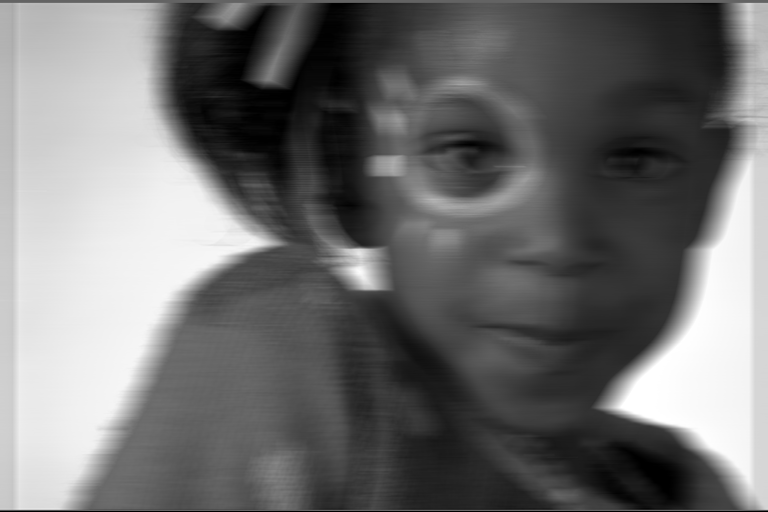
\includegraphics[width=0.45\textwidth]{source\_code/kodim15_b.png}
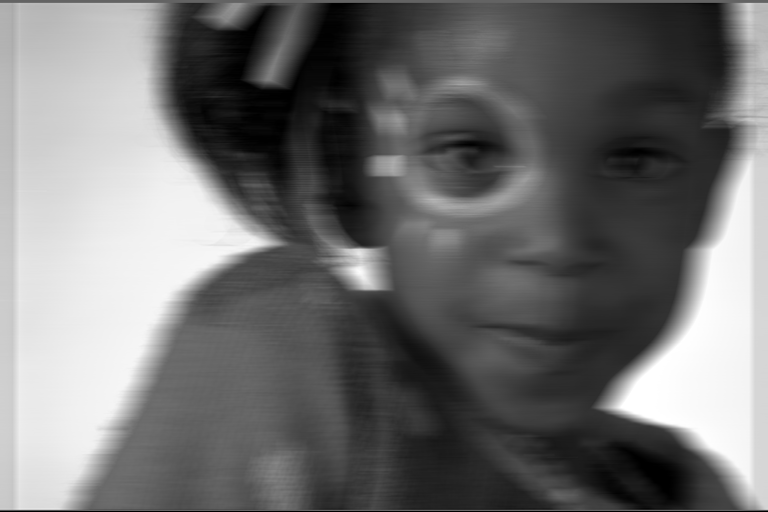
\includegraphics[width=0.45\textwidth]{source\_code/kodim15_b_result.png}
\item[c)] The file \texttt{images/kodim15c.png} was also distorted with some sort of blurr filter. Estimate the parameters of the filter as precisely as possible.
\item[d)] Describe the procedure you used for estimating the distortion. \\
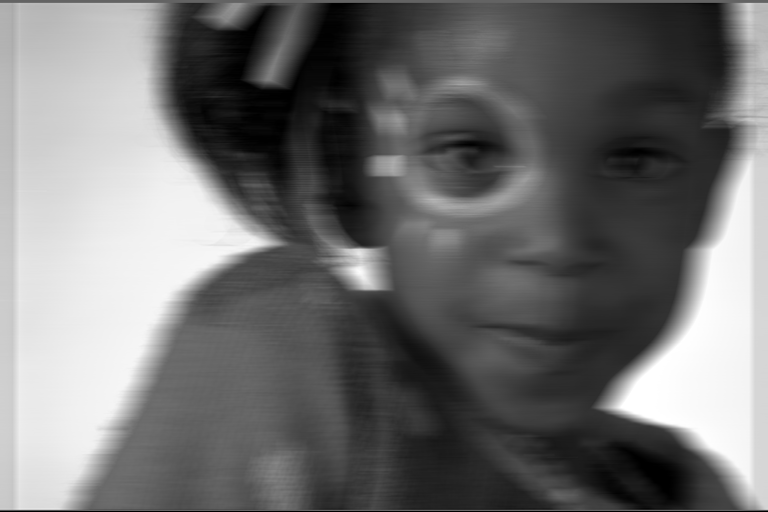
\includegraphics[width=0.45\textwidth]{source\_code/kodim15_b.png}
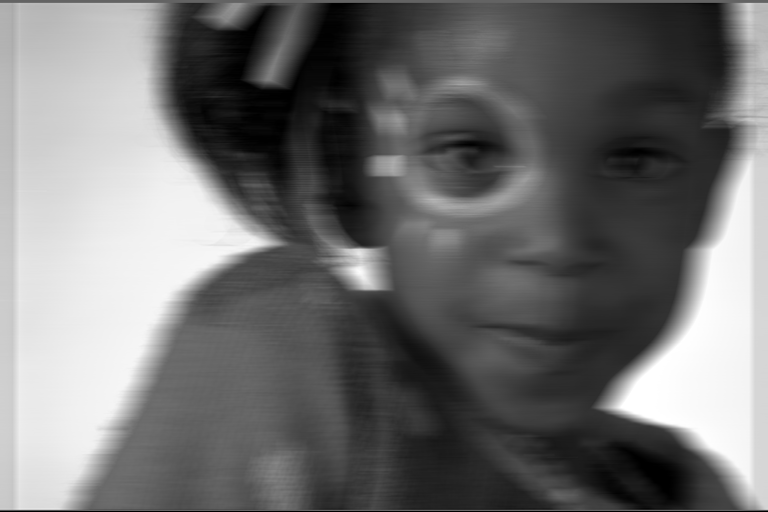
\includegraphics[width=0.45\textwidth]{source\_code/kodim15_b_result.png}

\end{enumerate}

\end{document}